\documentclass{beamer}
%\usepackage[cp1251]{inputenc}
%\usepackage[russian]{babel}
\usepackage{amsmath,mathrsfs,mathtext}
\usepackage{graphicx, epsfig}
\usetheme{Warsaw}%{Singapore}%{Warsaw}%{Warsaw}%{Darmstadt}
\usecolortheme{sidebartab}
\definecolor{beamer@blendedblue}{RGB}{15,120,80}

%%% Работа с русским языком
\usepackage{cmap}					% поиск в PDF
\usepackage{mathtext} 				% русские буквы в формулах
\usepackage[T2A]{fontenc}			% кодировка
\usepackage[utf8]{inputenc}			% кодировка исходного текста
\usepackage[english,russian]{babel}	% локализация и переносы

%% Beamer по-русски
\newtheorem{rtheorem}{Теорема}
\newtheorem{rproof}{Доказательство}
\newtheorem{rexample}{Пример}

%%% Дополнительная работа с математикой
\usepackage{amsmath,amsfonts,amssymb,amsthm,mathtools} % AMS
\usepackage{icomma} % "Умная" запятая: $0,2$ --- число, $0, 2$ --- перечисление

\usepackage{graphicx} % Allows including images
\usepackage{animate}
\usepackage{booktabs} % Allows the use of \toprule, \midrule and \bottomrule in tables

%----------------------------------------------------------------------------------------
%	TITLE PAGE
%----------------------------------------------------------------------------------------

%\title{Определение местоположения с помощью инерционных датчиков} % The short title appears at the bottom of every slide, the full title is only on the title page

\title[\hbox to 56mm{Определение местоположения  \hfill\insertframenumber\,/\,\inserttotalframenumber}]
{Определение местоположения с помощью инерционных датчиков}

\author[Макаров~М.\,, Зайнулина~Э.]{Макаров~М.\,, Зайнулина~Э.\,, Киселёва~Е.\,, Фатеев~Д.\,,
    Божедомов~Н., Толканев~А.\,, Ночевкин~В.,
    Протасов~В., Рябов~А.} % Your name
\institute[МФТИ] % Your institution as it will appear on the bottom of every slide, may be shorthand to save space
{\large
Московский физико-технический институт \\ % Your institution for the title page
\medskip
\textit{} % Your email address
}
%\date{\today} % Date, can be changed to a custom date
\date{\footnotesize{\emph{Курс:} Численные методы обучения по прецедентам\par (практика, В.\,В. Стрижов)/Группа 694, весна 2019}}
\begin{document}

\begin{frame}
\titlepage % Print the title page as the first slide
\end{frame}

\begin{frame}
\frametitle{Цель работы: повысить точность геопозиционирования} % Table of contents slide, comment this block out to remove it
\begin{block}{Задача}
    Позиционирование телефона в помещениях при условиях, когда глобальная навигационная система не может быть задействована, используя только инерционные датчики и данные о расположении телефона.
\end{block}

\begin{block}{Проблема}
    Значение инерциальных измерительных модулей (IMU) неточно, поэтому двойное интегрирование сигнала даёт траекторию, 
    значительно отклоняющуюся от истинной.
\end{block}

\begin{block}{Метод решения}
    Использовать априорные знания о расположении телефона для регрессии векторов скорости.
\end{block}
\end{frame}

%----------------------------------------------------------------------------------------
%	PRESENTATION SLIDES
%----------------------------------------------------------------------------------------

\begin{frame}
\frametitle{Траектория движения носителя телефона}
\begin{figure}[H]
    \centering
    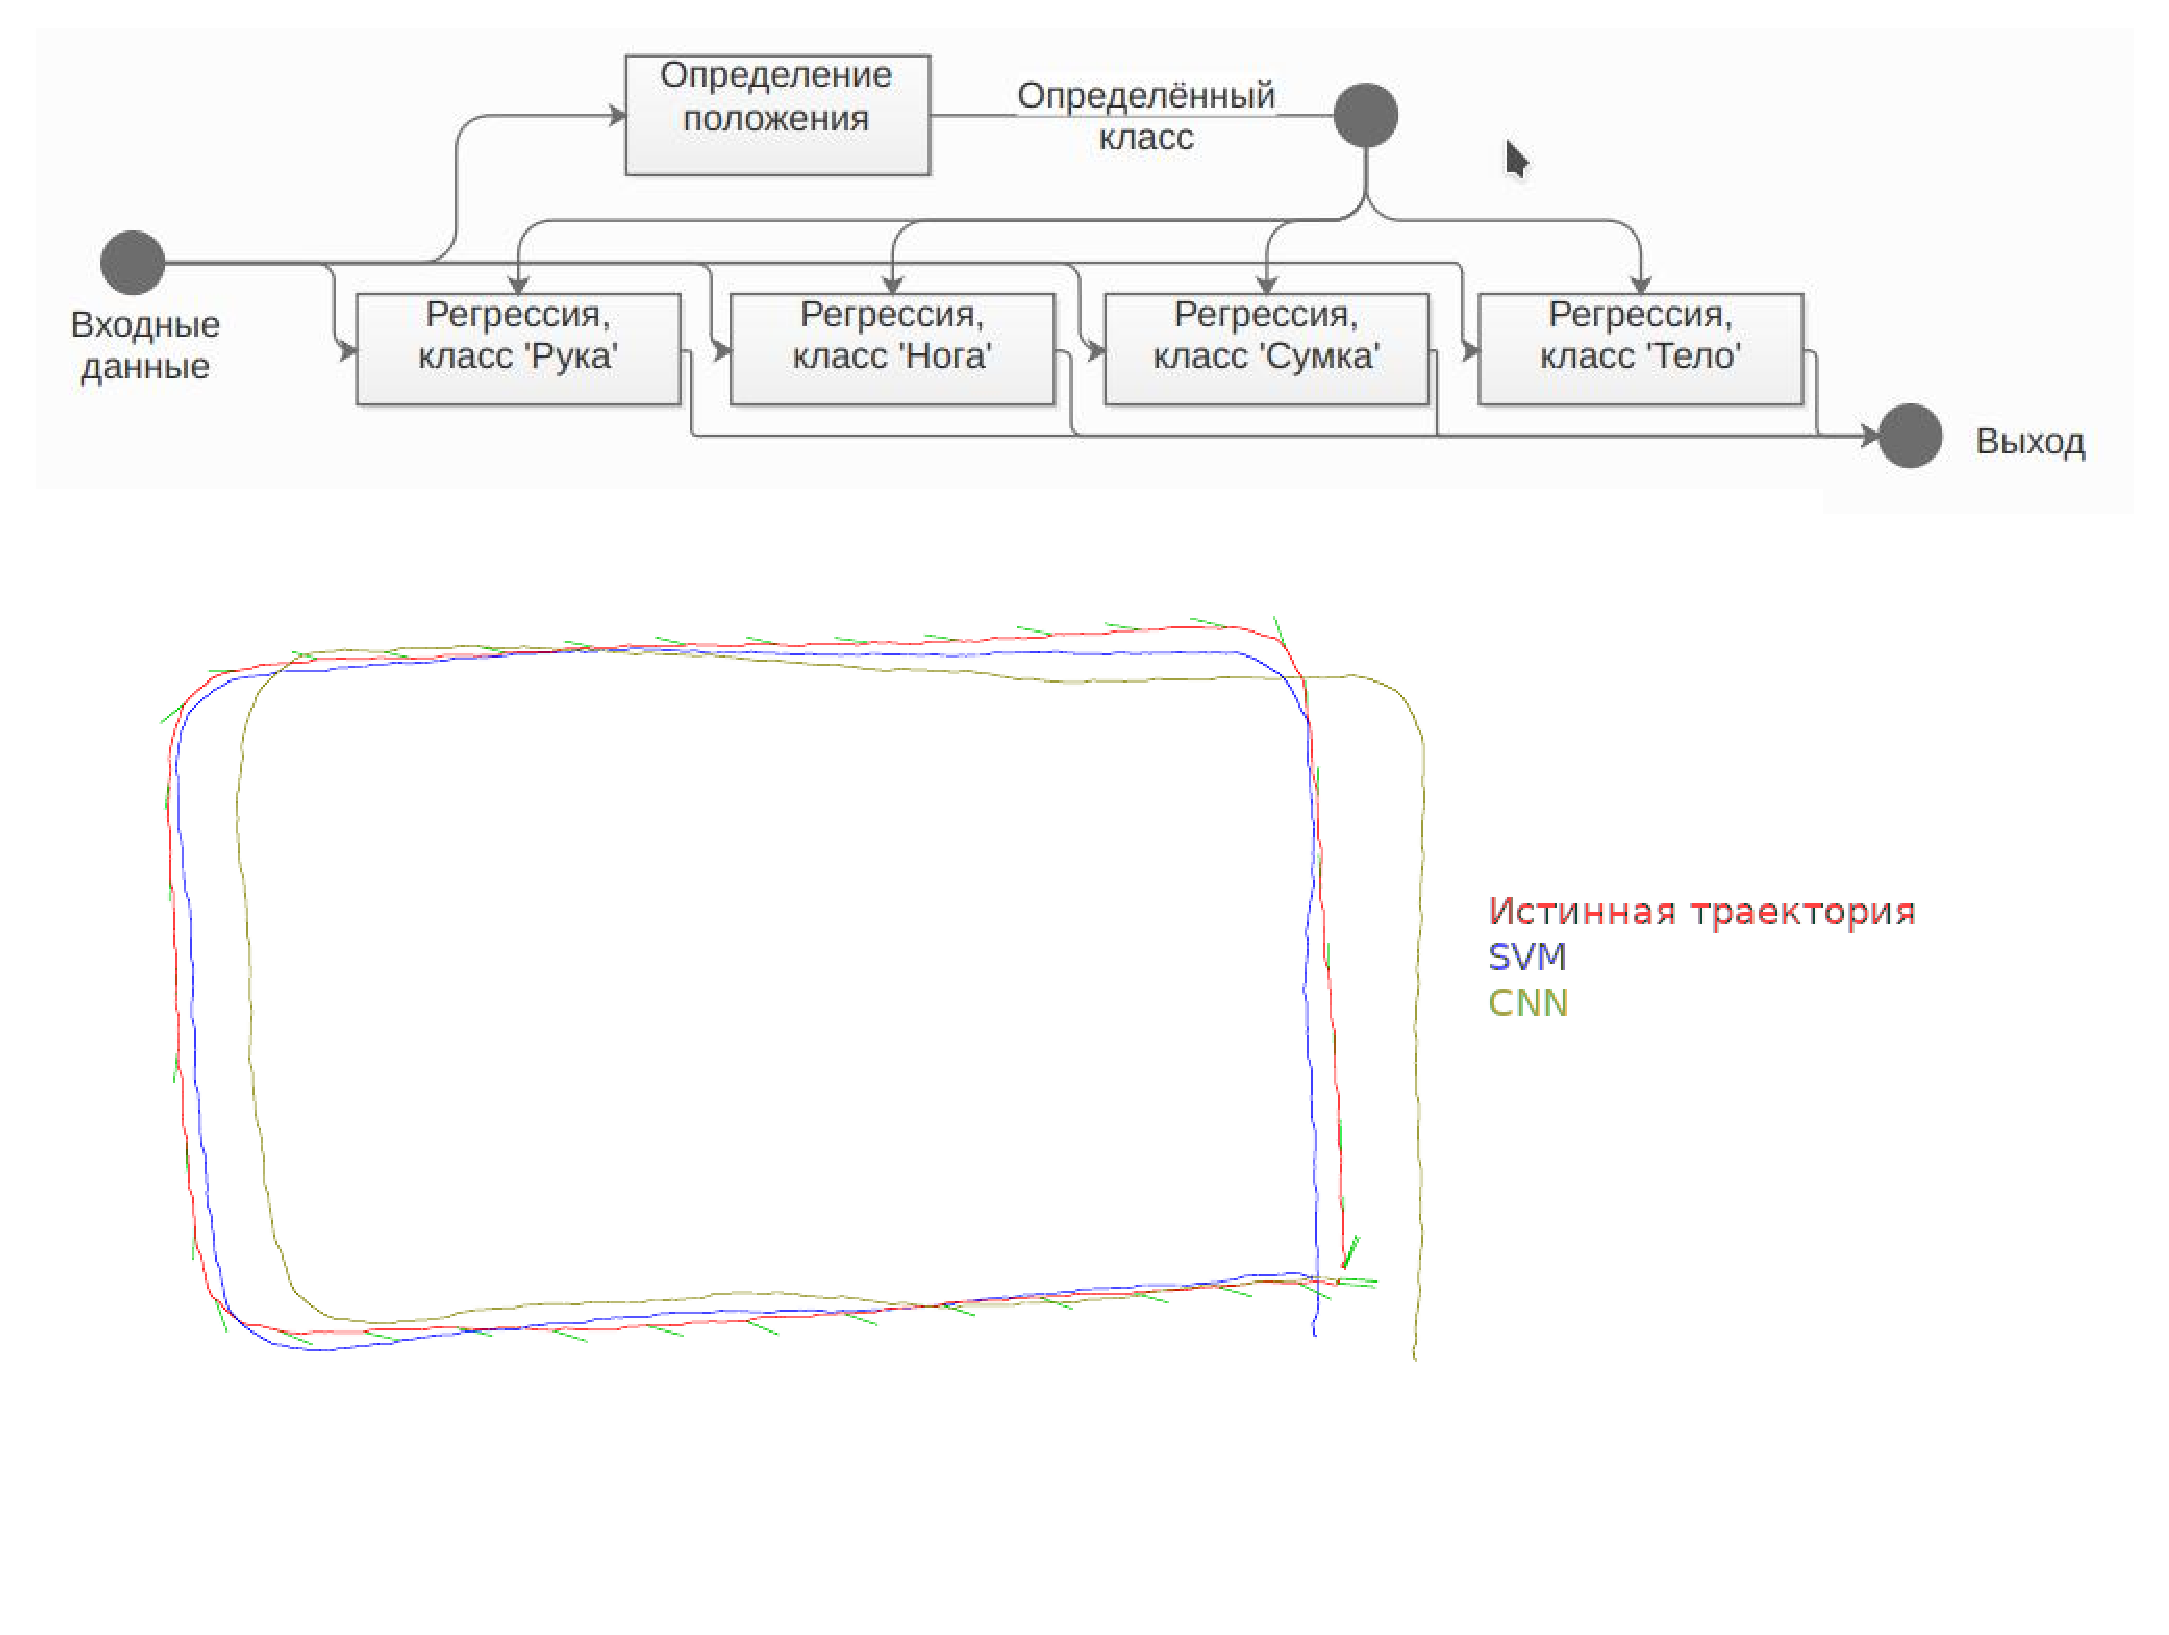
\includegraphics[scale=0.31]{images/title.eps}
\end{figure}
\end{frame}


\begin{frame}
\frametitle{Литература} % Table of contents slide, comment this block out to remove it
\begin{block}{Базовое решение}
    Hang Yan, Qi Shan, and Yasutaka Furukawa. Ridi: Robust imu double integration. CoRR, abs/1712.09004, 2017.
\end{block}
\begin{block}{Вычислительные эксперименты}
    Boyuan Wang, Xuelin Liu, Baoguo Yu, Ruicai Jia, and Xingli Gan. Pedestrian dead reckoning
based on motion mode recognition using a smartphone. Sensors, 18(6):1811, 2018.
\end{block}
\end{frame}

%---------------------------------------------------
\begin{frame}
\frametitle{Постановка задачи}
\begin{block}{Структура данных}

%$$ \mathrm{f}  : \mathrm{X}   \rightarrow \mathrm{Y}$$

$\mathbf{x} \in \mathbb{R}^{N \times T} $ --- признаки объекта --- угловые скорости и линейные ускорения в стабилизированной системе координат датчиков. Частота снятия данных --- 200 Гц

$\mathbf{y} \in \mathbb{R}^{2 \times T}$ --- траектория пешехода, 
$\mathbf{v}(t)$ --- скорость пешехода, $p(t) \in  P = \{0, 1, 2, 3\}$ --- рука, нога, сумка, туловище --- положение телефона.

В подзадачах классификации и регрессии $\mathbf{x}$ разбивается на перекрывающиеся отрезки времени $\mathbf{x}_i$ длины $windowsize$ (200) которые играют роль признаков, а $\mathbf{v}_i, p_i$ --- класс и положение в конечный момент отрезка $\mathbf{x}_i$ --- объектов. 
\end{block}

\end{frame}

%------------------------------------------------

\begin{frame}
\frametitle{Постановка задачи}
\begin{block}{Подзадачи}
\begin{enumerate}
\item Определить класс $p$ --- положения телефона --- моделью $f_1$. 
\item С помощью модели $f_2(\cdot, p)$ найти скорости.
\item Скорость интегрируется для получения траектории
%\[f = f_2 \circ f_1\]
%\[f_1: X \to P = \{0, 1, 2, 3\}\]
%\[f_2: X \times P \to Y\]
\end{enumerate}
\end{block}

\begin{block}{Оценка качества модели}
    \begin{enumerate}
        \item Точность предсказания класса 
        \item Сумма квадратов отклонений предсказанных скоростей от истинных
%        \item Корреляция между предсказанной и истинной траекториями пешехода.
    \end{enumerate}
    
\end{block}

\end{frame}
%----------------------------------------------------------------------------------------

\begin{frame}
\frametitle{Базовый эксперимент} % Table of contents slide, comment this block out to remove it
\begin{block}{Цель}
    Сравнить поведение различных моделей в каждой из подзадач. % при различных уровнях вычислительной сложности.
     Подобрать оптимальные гиперпапаметры.
\end{block}

\begin{block}{Данные}
    Данные взяты из \footnote{Hang Yan, Qi Shan, and Yasutaka Furukawa. Ridi: Robust imu double integration. CoRR, abs/1712.09004, 2017.}. 
    Траектории сняты при 4 различных положениях телефона и с нескольких людей.
    
    Также используются свои данные, снятые с другой модели телефона, но без истинной траектории.
\end{block}

%\begin{block}{Оптимизируемые параметры}
%Был произведён поиск по сетке коэффициента штрафа $C$ и $\gamma$:
%\begin{itemize}
%    \item $C \in [1, 10]$,
%    \item $\gamma \in [0.0001, 0.001, 0.01, 0.1]$.
%\end{itemize}

%Качество получаемых моделей измерялось с помощью кросс-валидации.
%\end{block}
\end{frame}

%------------------------------------------------

%\begin{frame}
%\frametitle{Базовая модель}
%    \begin{figure}[H]
%    \includegraphics[scale=0.5]{index.png}
%    \end{figure}
%\end{frame}

%\begin{frame}
%\frametitle{Базовая модель}
%\begin{block}{Корректировка предсказанных скоростей}
%\[\min_{\{x^1_I, x^{51}_I,\dots\}}V_{bias}=
%\min_{\{x^1_I, x^{51}_I,\dots\}}\sum_{f \in F_2}\|v_C^F-v_R^f\|+
%\lambda\sum_{f \in F_1}\|x^f_I\|^2,\]
%\[v_C^f = R_{SW}^f\sum_{f'=1}^f R_{WI}^{f'}(a_I^{f'}+x_I^{f'}),\]

%где $x^f_I$ - смещение ускорения, $f$ - единица блока выборки, $F$ - блок выборки, $v_C^F$ - скорректированное значение скорости, $v_R^f$ - %предсказанное значение скорости, $I$ - система координат устройства, $W$ - глобальная система координат, $S$ - IMU-стабилизированная система %координат, $R_{AB}$ - матрица перехода из системы координат $B$ в систему координат $A$.
%\end{block}
%\end{frame}

\begin{frame}
\frametitle{Рассматриваемые модели}
\begin{block}{Метод, используемый в базовом решении}
    \begin{itemize}
        \item SVM-классификатор и SVM-регрессор с гауссовским ядром
        \item Использовалась предобученная модель.
    \end{itemize}
    %\[\text{Ядро:} \quad K(x,x')=\exp{(-\gamma\|x-x'\|^2)}\]
\end{block}

\begin{block}{Метод ближайших соседей}
    \begin{itemize}
        \item kNN-классификатор и kNN-регрессор
        \item Метрика --- $l_1$, число соседей --- $5$, веса --- расстояние.
    \end{itemize}
\end{block}
\begin{block}{Свёрточные нейронные сети}
    \begin{itemize}
        \item Классификация --- 3 свёрточных слоя, 2 полносвязных
        \item Регрессия --- 3 свёрточных слоя, 4 полносвязных
    \end{itemize}
\end{block}
\end{frame}

%----------------------------------------------------------------------------------------

\begin{frame}
\frametitle{Сравнение моделей} % Table of contents slide, comment this block out to remove it
%\begin{itemize}

\begin{table}[H]
    \caption{Точность классификации и среднеквадратичная ошибка регрессии скорости на валидации}
    \begin{center}
        \begin{tabular}{|c|c|c|c|c|}
            \hline
            & & & \multicolumn{2}{c|}{Размер, в мб} \\
            \cline{4-5}
            \raisebox{1.5ex}[0cm][0cm]{Модель}
            & \raisebox{1.5ex}[0cm][0cm]{Точность}
            & \raisebox{1.5ex}[0cm][0cm]{Ошибка} 
            %& $\gamma=0.1$
            & классификатор
            & регрессоры
            %& $\gamma=0.1$ 
            \\
            \hline
            SVM
            & $0.379$ 
            & $0.085$ 
            & $30$
            & $130$
            \\
            \hline
            kNN
            & $0.372$
            & $0.027$
            & $260$
            & $260$
            \\
            \hline
            CNN
            & $0.381$
            & $0.013$
            & $0.006$
            & $0.8$
            \\
            \hline
            
        \end{tabular}
    \end{center}
\end{table}
Заметьте, что средняя скорость движения $\sim 1.1$ м/с.
%\end{itemize}
\end{frame}


%----------------------------------------------------------------------------------------
\begin{frame}
\frametitle{Своя выборка} % Table of contents slide, comment this block out to remove it
%\begin{itemize}

\begin{figure}[h]
\centering
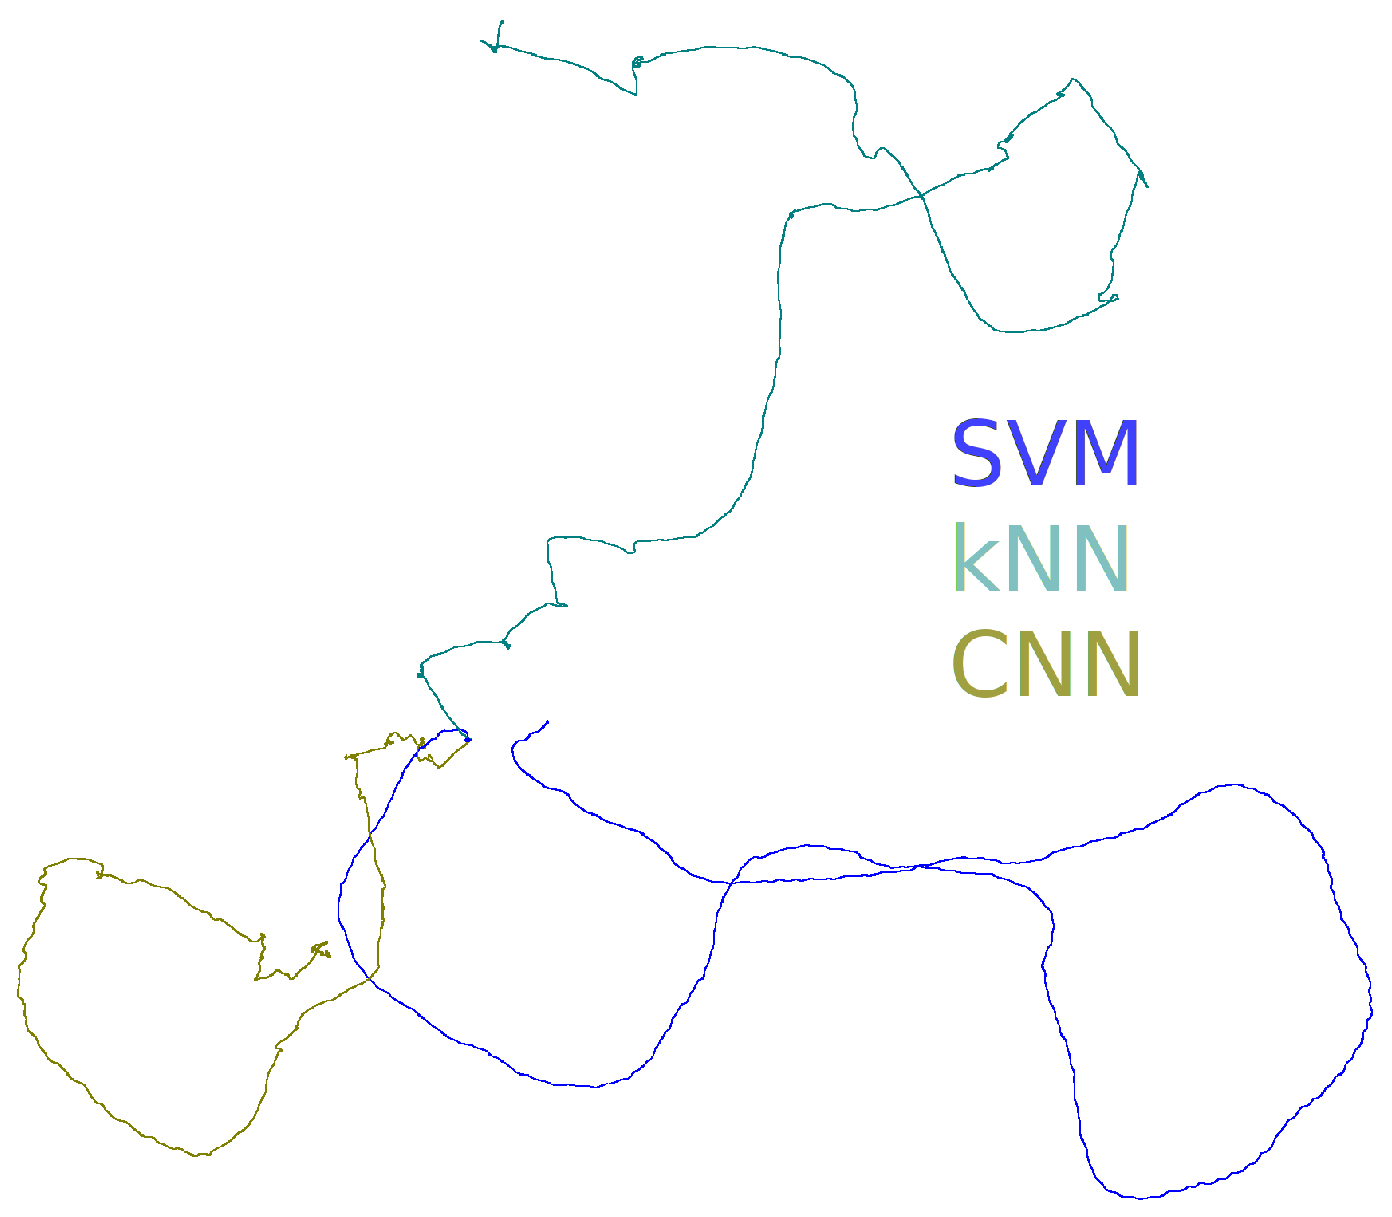
\includegraphics[scale=0.3]{images/traj.eps}
\end{figure}
В отличие от остальных моделей на нашей выборке SVM показывает хороший результат.

%\end{itemize}
\end{frame}

%----------------------------------------------------------
\begin{frame}
\frametitle{Выводы}
\begin{block}{Выводы}
\begin{itemize}
\item Все модели обладают невысокой точностью классификации, что скорее всего вызвано недостатком данных.
\item Также несмотря на то, что среднеквадратичная ошибка регрессии у CNN и kNN ниже, качество восстановленной траектории значительно хуже, чем у SVM.
Это означает, что она не подходит для сравнения моделей.
\end{itemize}
\end{block}

\begin{block}{Дальнейшее развитие}
    \begin{itemize}
    \item Собрать больше данных для увеличения качества.
    \item Придумать способы генерации синтетических данных из существующих
    \end{itemize}
\end{block}
\end{frame}



%-------------------------------------------------------
\end{document}